\documentclass[12pt,a4paper]{article}

\usepackage{a4wide}
\usepackage{fancyhdr}
\usepackage{graphicx}
\usepackage{epsfig}
\usepackage{parskip}
\usepackage[ansinew]{inputenc}
\usepackage{amsmath}
\usepackage{amssymb}
\usepackage{bm}
\usepackage[free-standing-units=true]{siunitx} % for consistent handling of SI units
\usepackage[colorlinks=true, pdfstartview=FitV, linkcolor=blue, citecolor=blue, urlcolor=blue]{hyperref} % enable links

\setlength{\parindent}{0pt}

\newcommand{\m}[1]
{\mathrm{#1}}

\title{Experiment 15 - Wavelength Measurements with a Grating}
\author{Cedric Renda, Fritz Kurz}
\date{\today }

\begin{document}

\maketitle
\begin{abstract}
The abstract is a short summary of the experiment. It should
motivate the reader to actually read the whole paper. The length of
the abstract should not exceed 10 lines. Every section of the report
should be represented by one or two sentences. This includes the
results and the conclusions. There is no need to keep the reader in
suspense over the findings that you want to present. Often the
abstract is written last.
\end{abstract}



\tableofcontents

\section{Introduction}

In this experiment we want to use the universal gas equation \cite{gas}
\begin{equation}
	\displaystyle PV=nRT
	\label{eq::gas}
\end{equation} were $P$ is the pressure, $V$ the volume, $n$ the number of particles, $R$ universal gas constant and $T$ the temperature, to determine the lowest limit of the so called thermodynamic Celsius temperature scale.
At this lowest point of temperature the enthalpy and entropy of a cooled ideal gas reaches its minimum values.
By definition this point is the zero point of the SI base unit of temperature Kelvin, which is defined as follows \cite{kelvin}:
\begin{itemize}
	\item The kelvin, symbol K, is the SI unit of thermodynamic temperature. It is defined
	by taking the fixed numerical value of the Boltzmann constant $k$ to be
	$1.380 649 \times 10^{-23}$ when expressed in the unit \si{\J}$\si{\K}^{-1}$, which is equal to $\si{\kg}$ $\si{\m}^2$ $\si{\s}^{-2}$ $\si{\K}^{-1}$,
	where the kilogram, metre and second are defined in terms of $h$, $c$ and $\Delta vC_s$.
\end{itemize}
 
In the process to find this coldest temperature possible in the absolute temperature, we use a glass bulb filled with a known gas, a pressure sensor and two well known temperatures to measure and calculate the zero point. 
Once the pressure and temperature of the gas in the glass bulb is known, all kinds of temperatures can be measured with the change of pressure in the sealed glass bulb.
To show this the temperature of liquid nitrogen is measured at the end of the experiment.
%\begin{figure}[Ht]
%	\centering
%	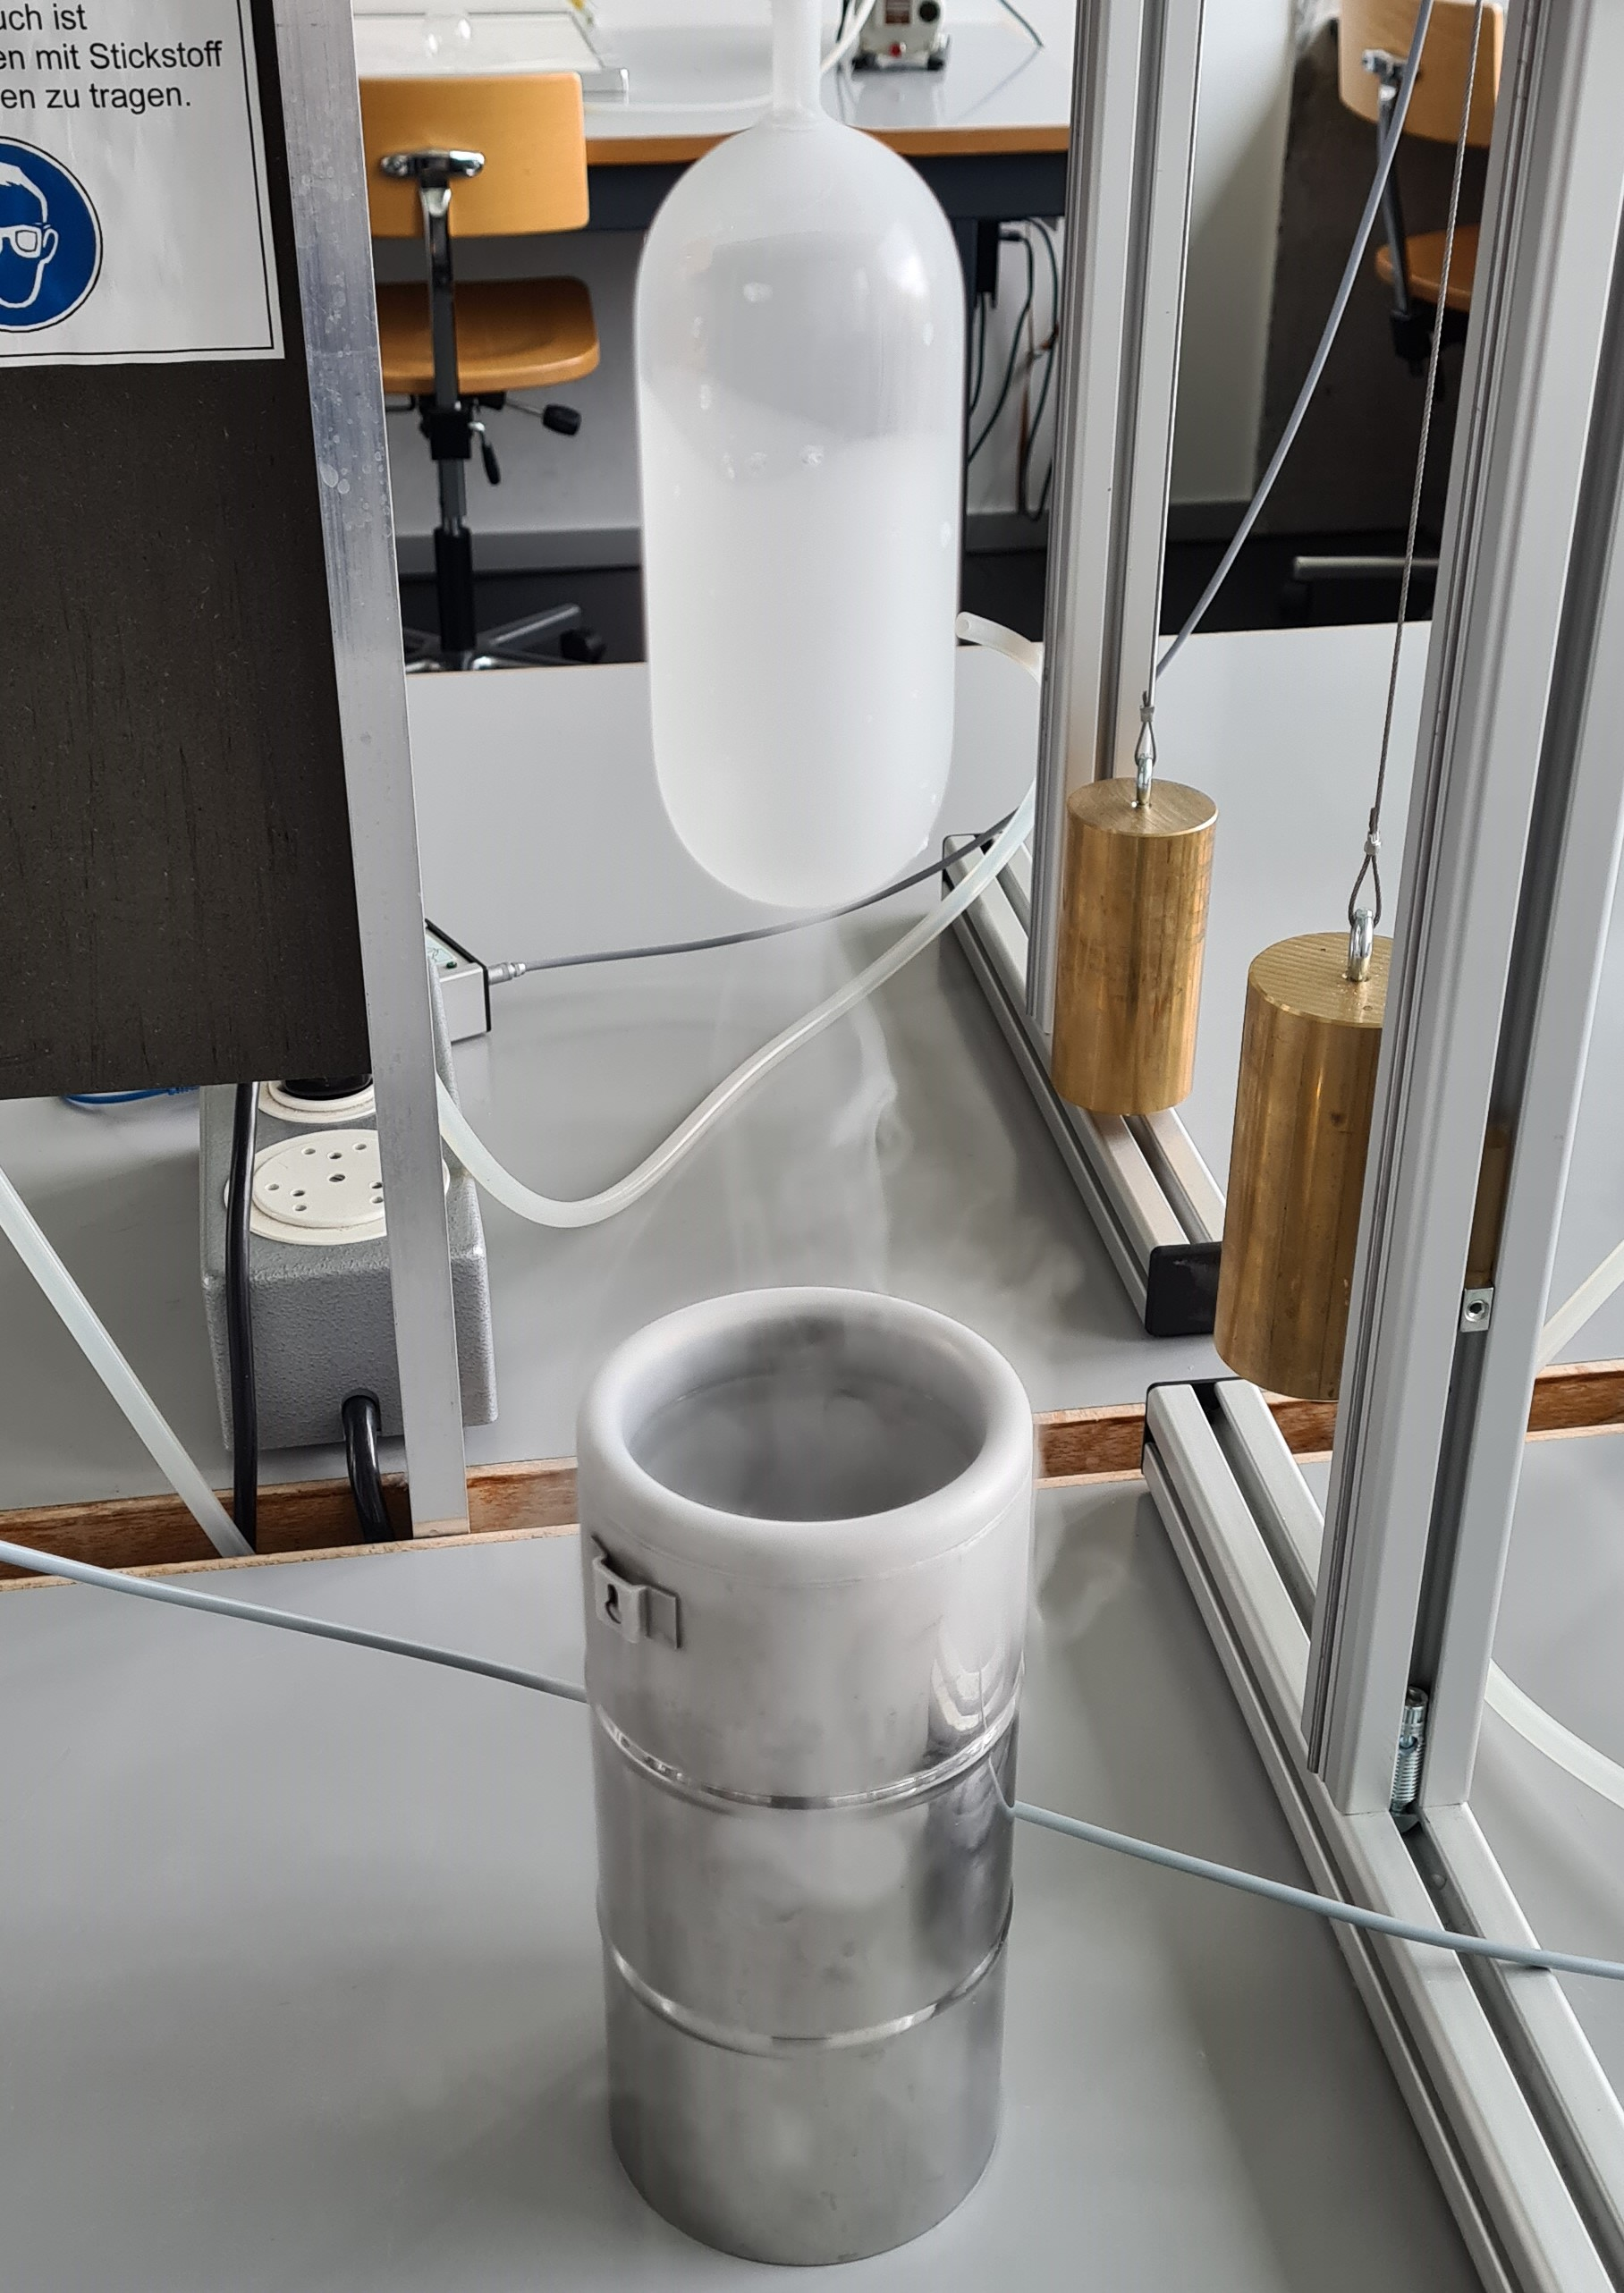
\includegraphics[width=0.5\textwidth]{sections/images/liquid.jpg}
%	\caption{Sealed glass bulb filled with helium after being put in liquid nitrogen to measure the temperature of liquid nitrogen.}
%\end{figure}

\section{Simple Measurement with He}
\subsection{Experiment}
In this part of the experiment we want to use the dampened natural oscillation of our system to determine the dampening constants $\alpha_{1, 2, 3}$.
The formula for the amplitude of this system with a given starting value $A_0$ is  as follows.
\begin{align}
	A(t) = A_0 e^{-\alpha t}
	\label{eq::model}
\end{align} 
To determine $\alpha$, we can measure the amplitude of the system for different times $t$, and then fit the model (\ref{eq::model}) to our measurement points numerically.

We always start with an amplitude $A_0$ of $110 \pm 0.5 \degree$.
For the first dampening $\alpha_1$ with $I_1 = 0.64 \pm \SI{0.01}{\ampere}$, we measure the amplitudes $A$ at every third period, for $n_1 = 24$ periods in total.
As a higher dampening results in a faster decay time, we measure $n_2 = 14$ periods with $I_2 = \SI{0.9}{\ampere}$, measuring every second period, and $n_3 = 8$ periods for $I_3 = \SI{1.2}{\ampere}$, measuring every single period.
For every dampening, we also measure the total time $t_i$ of those $n_i$ periods with a stopwatch. We estimate the error of every measurement for $t$ with $\Delta t = \SI{0.4}{\second}$ because of the human reaction time.


\subsection{Results}

The measurements of the characteristic curve of the detector are shown in Fig. \ref{fig::plateau}, together with the fit to the Geiger plateau, which will be explained later.
The middle of the plateau is at around \SI{740}{\volt}, so we will operate the system at this voltage for the rest of the experiment.

\begin{figure} [ht]
	\centering
	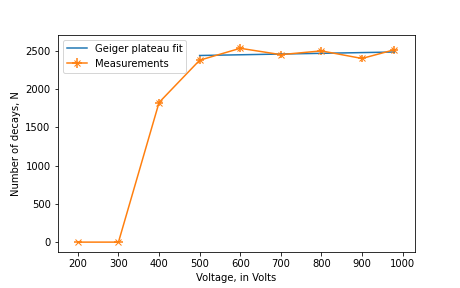
\includegraphics[width=400pt]{python/plateau.PNG}
	\caption{Number of counts plotted against voltage for duration of \SI{30}{\second}. Uncertainty only on voltage.}
	\label{fig::plateau}
\end{figure}

The uncertainty of the number of counts is described by the Poisson-distribution, therefore the uncertainty on any count is $\Delta N = \sqrt{N}$ \cite{manual}.
We measured an activity of $N = 7453 \pm  86$ decays, together with $N_{BG} = 50 \pm 7$ decays without the source.

As said, the distance is given as $d = 101 \pm \SI{0.5}{\milli\meter}$, and the diameter of the aperture we measured as $2*r = 18.05 \pm \SI{0.025}{\milli\meter}$.
\subsection{Data Analysis}

In the data analysis section you describe the post processing of the
data. How did you obtain the data that you plot in the figures? The raw data does not necessarily need
to be presented in the report. An important part of this paragraph
are the measurement uncertainties. You should provide the
uncertainties of all experimental results, i.e. in the form of error
bars. Further, you should explain the origin of these uncertainties.

There are many way how you can include equations and mathematical terms in your report. The easiest is to write them inside the text like this: $\Gamma =\SI{1.5}{\micro\meter\per\square\second}$. If you need to write a long equation, it is recommended to use e.g. the align environment.
\begin{align}
    \Gamma = \frac{a}{4\kappa}\times ...
\end{align}

All figures or tables that are part of your report have to be
referenced somewhere in the text, ideally in order of their
appearance (``as shown in Fig. \ref{fig1}''). Figures have to
have axis labels with units and a sensible scale. If more than on
data set is plotted you need to provide a legend. This may be a sentence in the caption (``red dots denote data measured with \SI{1}{\milli\volt}, blue crosses were measured with \SI{10}{\milli\volt}'').

After you have presented the data you need to interpret it. To this
end you want to discuss the theoretical model that describes your
data and you will derive model parameters from your measurement data
(i.e. by fitting it to the data). Here, you will again elaborate on
the confidence interval of the derived values (error propagation).
This is an important part of the report and it will be the basis for
the next paragraph.
\section{Precision Measurement with Hg}
\subsection{Experiment}
In this second part of the experiment we precisely measure the wavelengths of the mercury spectrum with a grating spectrometer.
First we had to First, we had to adjust the telescope correctly, according to the procedure given by the manual\cite{manual}.
The setting includes the following five steps described in the manual \cite{manual}:
\begin{itemize}
	\item Focusing the telescope to infinity
	\item Vertical alignment of the telescope axis to the spectrometer axis
	\item Adjusting the collimator
	\item Vertical alignment of the grating to the collimator axis
	\item Adjusting the grating
\end{itemize}


\subsection{Results}

Results of second part.
\subsection{Analysis}


\section{Conclusion and Discussion}

So far you have discussed how you have obtained your data and the
quantities you derived from it. In this section you should discuss
the results in the context of physical laws. Depending on the
experiment you want to compare your result and its uncertainty with
the literature value. If you want to confirm a physical model that
explains a certain phenomenon you want to assess if this model
describes the data well within the confidence intervals, or whether
a simpler model describes the data just as well.
\section{Conclusion}
The first method is not very good to evaluate exact values. 
But it is suitable to get an rough estimate of the searched spectrum and its wavelengths.

If we want to make this method more exact the distances and positioning as well as the scales have to be more exact. 
In conclusion it is a very easy setup which leads in very rough approximations on the searched values.



For the method used to get the Hg spectrum it would be important to get a better estimation of sources of error.
This means that the calibration of the apparatus have to be done multiple times to see how big the effects are on the results. 
Furthermore it would help to measure the starting and ending point of an light line to see where the middle lays.
This would remove another error source coming from measuring the wrong angle.

On the whole there is potential in doing more precise measurements with this second method. 
It just have to be done very carefully and multiple times to remove as many errors as possible.

\newpage

\begin{thebibliography}{99}

% =======================================================================================
% =======================================================================================

\bibitem{manual}
Lab manual 41 - Beta Decay, Physikpraktikum der ETH Zurich,  \url{https://ap.phys.ethz.ch/Anleitungen/Bilingual/41_Manual.pdf}.


\end{thebibliography}




\end{document}